\documentclass[ddcfooter, aspectratio=169, hyperref = {colorlinks,bookmarks=true,citecolor=blue,urlcolor=blue}]{beamer}
\usepackage[utf8]{inputenc}  % Kodierung der Datei
\usepackage[T1]{fontenc}  % Vollen Umfang der Schriftzeichen
\usepackage{amsmath}
\usepackage{amssymb}
%\usepackage{nameref}
\usepackage{isomath}
\usepackage{upgreek}
\usepackage{caption}
\usepackage{bbm}
\usepackage{mathtools}
\usepackage{mathrsfs}

\usepackage{comment}

%\usepackage{hyperref}
%\usepackage[colorlinks,bookmarks=true,citecolor=blue,linkcolor=red,urlcolor=blue]{hyperref}


\usepackage{bm}
\usepackage{bbm}

\usepackage{subfig}
%\usepackage{floatrow}

%sinnvolle Abstände im Inhaltsverzeichnis
\makeatletter
\patchcmd{\beamer@sectionintoc}
  {\vfill}
  {\vskip\itemsep}
  {}
  {}
\makeatother  

% Custom command to obtain the currently active label (of section, subsection etc.)
\makeatletter
\newcommand*{\currentname}{\@currentlabelname}
\makeatother

\newcommand\blfootnote[1]{%
  \begingroup
  \renewcommand\thefootnote{}\footnote{#1}%
  \addtocounter{footnote}{-1}%
  \endgroup
}

%Bilder neben Text
\newcommand{\lenitem}[2][.7\linewidth]{\parbox[t]{#1}{\strut #2\strut}}

\usetheme{Frankfurt}
\usecolortheme{beaver}
\setbeamertemplate{footline}[frame number]
\setbeamertemplate{navigation symbols}{}
\setbeamertemplate{headline}{}


\title[]{Quantum Hall Effect without Chern Bands}
\author{\texorpdfstring{\textbf {Benjamin Michen} (TU Dresden) \\
Jan Carl Budich (TU Dresden, MPIPKS), \newline \vspace{10pt} Contact: \url{benjamin.michen@tu-dresden.de}}{}}
\date{March 12, 2026}

\titlegraphic{
\raisebox{-0.5\height}{\includegraphics[width=3cm]{Illustrations/TUD_logo}}\hspace*{4.75cm}~%
\raisebox{-0.5\height}{\includegraphics[width=2cm]{Illustrations/MPIPKS_logo.png}}
}

% Insert slide with section name before each section
\AtBeginSection[]{
  \begin{frame}
  \vfill
  \centering
  \begin{beamercolorbox}[sep=8pt,center,shadow=true,rounded=true]{title}
    \usebeamerfont{title}\thesection~ \insertsectionhead\par%
  \end{beamercolorbox}
  \vfill
  \end{frame}
}


\begin{document}
\maketitle

\section{Background: Some Facts about the Quantum Hall Effect}

\begin{frame}
\frametitle{\insertsectionhead}
\textbf{\large Hall conductance as a function of Fermi energy} \\
\vspace{0.5em}
For translation-invariant system with Bloch Hamiltonian $H(\bm k)$, eigenvectors $|u(\bm k) \rangle$, energies $E_{\bm k}$, and Berry curvature $\mathcal F = i [\langle \partial_{k_x} u| \partial_{k_y} u \rangle - \langle \partial_{k_y} u| \partial_{k_x} u \rangle]$, we have:
\begin{align}
\sigma_{xy}(E_\mathrm{F}) = \frac{e^2}{h} \frac{1}{2\pi}\int_{E_{\bm k}<E_\mathrm{F}}\mathrm{d}^2k \,  \mathcal F. \nonumber
\end{align}

\begin{itemize}[<+(1)->]
\item For $E_\mathrm{F}$ in spectral gap, $\sigma_{xy}$ equals Chern number $\Rightarrow$ integer quantum Hall effect.
\item For $E_\mathrm{F}$ in band spectrum, $\sigma_{xy}$ takes continuous values.
\item Random disorder creates mobility gap $\Rightarrow$ forces  integer value of $\sigma_{xy}$ at any $E_\mathrm{F}$!
\end{itemize}
\end{frame}



\begin{frame}
\frametitle{\insertsectionhead}
\textbf{\large Two-parameter conductance scaling in the presence of disorder} \\
%\vspace{0.5em}
	\begin{figure}[htp!]	 
			\centering 
			\includegraphics[trim={0cm 0cm 0cm 0.5cm}, width = 0.9 \linewidth]{Illustrations/2_param_scaling_DPG/2_param_scaling_DPG.png} 			
	\end{figure}\blfootnote{D. E. Khmelnitskii, \em{Quantization of Hall conductivity}, 
\href{http://jetpletters.ru/ps/1485/article_22668.shtml}{ZhETF Pisma Redaktsiiu {\bfseries{38}} (1983)}}
\vspace{-1.5em}
\begin{itemize}[<+(1)->]
\item Scaling theory depends on forward ($\sigma_{xx}$) and transverse ($\sigma_{xy}$) conductance.
\item Non-integer values of $\sigma_{xy}$ rounded to the nearest integer in thermodynamic limit!
\end{itemize}

\end{frame}


\begin{comment}
\begin{frame}
\frametitle{\insertsectionhead}
\textbf{\large Conductance scaling in the presence of disorder} \\
%\vspace{0.5em}
	\begin{figure}[htp!]	 
			\centering 
			\includegraphics[trim={0cm 0cm 0cm 0.5cm}, width = 0.9 \linewidth]{Illustrations/2_param_scaling_DPG/2_param_scaling_DPG.png} 			
			\caption*{Two-parameter scaling theory depends on forward ($\sigma_{xx}$) and transverse ($\sigma_{xy}$) conductance.}
	\end{figure}\blfootnote{D. E. Khmelnitskii, \em{Quantization of Hall conductivity}, 
\href{http://jetpletters.ru/ps/1485/article_22668.shtml}{ZhETF Pisma Redaktsiiu {\bfseries{38}} (1983)}}
\vspace{-1.5em}

\setbeamercolor{block body example}{bg=gray}
  \begin{exampleblock}{}
  \centering
	Disorder rounds $\sigma_{xy}$ to the nearest integer in the thermodynamic limit!
  \end{exampleblock}
  
\end{frame}
\end{comment}


\section{Quantum Hall Effect in a Model without Chern Bands}

\begin{frame}
\frametitle{\insertsectionhead}
\textbf{\large Method} \\
%\vspace{0.5em}
	\begin{figure}[htp!]	 
			\centering 
			\includegraphics[trim={0cm 0cm 0cm 0.5cm}, width = 0.9 \linewidth]{Illustrations/Fig_scattering_theory.png} 			
	\end{figure}
\vspace{-1.5em}
\begin{itemize}[<+(1)->]
\item Landauer-Büttiker formalism: quantum transport as scattering / wave matching problem
\item $S$-matrix elements calculated with Kwant\footnote{C. W. Groth, M. Wimmer, A. R. Akhmerov, X. Waintal, {\em Kwant: a software package for quantum transport}, \href{https://iopscience.iop.org/article/10.1088/1367-2630/16/6/063065}{New J. Phys. 16, 063065 (2014)}} package
\end{itemize}

\end{frame}

\begin{frame}
\frametitle{\insertsectionhead}
\textbf{\large Model} \\
\begin{align*}
\hat H = \underbrace{\sum_{\bm k} \bm c_{\bm k}^\dagger \left[h_0(\bm k)\right] \bm c_{\bm k}}_{\hat H_0} \;+ \;\underbrace{W\sum_{j_x, j_y} \sum_{\alpha = a,b} f_{\bm j, \alpha} c_{\bm j, \alpha}^\dagger c_{\bm j, \alpha}}_{\hat W},
\end{align*}

\begin{itemize}[<+(1)->]
\item $\hat H_0$ exhibits two topologically trivial bands\footnote{For completeness: explicit Bloch Hamiltonian is $h_0(\bm k) = \bm d(\bm k) \cdot \bm \sigma $ with coefficients $d_x(\bm k) = \gamma \sin(k_x)$, 
$d_y(\bm k) = \lambda(k_x) \sin(k_y)$,
$d_z(\bm k) = \gamma_2[r - \cos(2 k_x)] - \lambda(k_x) \cos(k_y)$, where $\lambda(k_x) =  \epsilon_1 + \epsilon_2 (1 - \cos(k_x))/2 $ and parameters $r = 1.5$, $\epsilon_1 = 0.3$, $\epsilon_2 = 2$, $\gamma  =2$, and $\gamma_2 = 0.3$.} but strong anomalous Hall effect with $\sigma_{xy} \geq 0.5 e^2 / h$!
\item Disorder potential $\hat W$ with overall strength $W \ge 0$ and random amplitudes $f_{\bm j, \alpha}$ drawn uniformly from $[-1,1]$.
\end{itemize}
\vspace{0.5em}
\end{frame}

\begin{frame}
\frametitle{\insertsectionhead}
\textbf{\large Disorder induces integer quantum Hall effect} \\
\vspace{0.5em}
\begin{figure}[htp!]	 
	\centering 
	\includegraphics[trim={0cm 0cm 0cm 0.5cm}, width = 0.9 \linewidth]{Illustrations/QHE_wo_CB_DPG/QHE_wo_CB_DPG.png} 			
	\caption*{(a) Band structure of $\hat H_0$. (b) Hall conductance without ($W = 0$) and with disorder ($W = 1.5$).} 
\end{figure}	
\end{frame}

\section{Edge Transport and Finite-Size Effects}

\begin{frame}
	\frametitle{\insertsectionhead}
\begin{columns}[onlytextwidth,T]
\begin{column}{.45\textwidth}
\begin{overlayarea}{\linewidth}{0.75\textheight}
\only<1-2>{
\textbf{\large Edge Transport} \\
\vspace{0.5em}	
	\begin{itemize}[<+->]
		\item Different geometries (planar/OBC vs. cylindrical/PBC) reveal edge state contribution
		\item Additional marker: winding number of reflection matrix over boundary angle
\begin{align*}
\nu = \frac{1}{2\pi} \oint_{0}^{2 \pi} \mathrm{d} \phi\, \left(\frac{\partial}{\partial\phi} \mathrm{ln}[\mathrm{det}(R)]\right) \label{Eqn:W_num}
\end{align*}
	\end{itemize}}

\only<3-5>{
\textbf{\large Finite size effects}	\\
\vspace{0.5em}	
	\begin{itemize}[<+(3)->]
		\item For $L \to \infty$, any $W > 0$ stabilizes IQH plateau
		\item $W \to 0$ means diverging localization length \\
		$\Rightarrow$ Order-of-limits problem between $W \to 0$ and $L \to \infty$
\end{itemize}
}
	
\end{overlayarea}
\end{column}	

\begin{column}{.55\textwidth}
\flushright
\begin{overlayarea}{\linewidth}{0.75\textheight}
\only<1>{%
  \includegraphics[trim={-0.1cm 0cm 2.5cm 1cm}, width=\linewidth]{Illustrations/2_terminal_DPG/2_terminal_DPG_no_nu.png}\\
  \captionof*{figure}{\hspace{1em}\parbox{\linewidth}{Two-terminal transport along $x$-direction for system size $N_x = 600$, $N_y = 150$. (a) OBC along $y$, (b) PBC along $y$. Inset: Finite size scaling.}}
}%
\only<2-5>{%
  \includegraphics[trim={-0.1cm 0cm 2.5cm 1cm}, width=\linewidth]{Illustrations/2_terminal_DPG/2_terminal_DPG_nu.png}\\
  \captionof*{figure}{\hspace{1em}\parbox{\linewidth}{Two-terminal transport along $x$-direction for system size $N_x = 600$, $N_y = 150$. (a) OBC along $y$, (b) PBC along $y$. Inset: Finite size scaling.}}
}%
\end{overlayarea}
\end{column}
\end{columns}
\end{frame}

\begin{frame}
\begin{block}{Paper}
\Large
  \begin{center}
B. Michen and J.C. Budich, \\{\em Quantum Hall Effect without Chern Bands}, \\ \href{https://journals.aps.org/prl/abstract/10.1103/dgd8-4gzf}{Phys. Rev. Lett. {\bfseries{135}} (18), 186603 (2025)}.
\end{center}
\end{block}
\blfootnote{Contact: \url{benjamin.michen@tu-dresden.de}}

\pause

\vfill
\centering
\Large{Thanks for your attention!}
\vfill
\Large{Questions?}
    
\end{frame}

\end{document}

\section{The fractional quantum Hall effect and the fractional Chern insulator}

\begin{frame}
\frametitle{\insertsectionhead}
\textbf{ \large The (fractional) quantum  Hall effect\\}

 
Consider a 2D electron gas in the $x,y$-plane subjected to a perpendicular magnetic field

\begin{align}
\bm B = B \bm e_z \nonumber
\end{align}

\pause
Vector potential in Landau gauge $\bm A = (0, Bx, 0)$ yields single-particle Hamiltonian 

\begin{align}
H = \frac{1}{2 m} \left (- i \hbar \frac{\mathrm{d} x}{\mathrm{d} x}\right  )^2 + \frac{1}{2 m} \left ( - i \hbar \frac{\mathrm{d} y}{\mathrm{d} y} + eB x\right  )^2 \nonumber
\end{align}

\pause
$\Rightarrow$ Eigenenergies form perfectly flat quasi bands, so-called Landau levels

\end{frame}

\begin{frame}
	\frametitle{\insertsectionhead}
	\begin{figure}[htp!]	 
			\centering 
			\includegraphics[trim={0cm 0cm 0cm 0cm},clip, width= 0.8 \linewidth]{Images/Landau_Levels.png} 
			\caption*{Landau levels for a system of size $L_x \times L_y$.}
	\end{figure}
\end{frame}

\begin{frame}
\frametitle{\insertsectionhead}

\pause
\begin{itemize}[<+->]
	\item Complete filling of the Landau levels leads to a transverse conductance 	
	\begin{align}
	\sigma_{x,y} = n \sigma_0, \; \; \; n \in \mathbbm{N} \nonumber
	\end{align}	
	 quantized in integers of $\sigma_0 = \frac{e^2}{2 \pi \hbar}$ \\
	 \vspace{10pt}
	 \centering $\Rightarrow$ Integer Quantum Hall Effect 
	 \vspace{10pt}
	\item Filling to a fraction $\nu = \frac{1}{m}$, may lead to a fractionalized quantization
	\begin{align}
	\sigma_{x,y} =  \frac{1}{m} \sigma_0  , \; \; \; m \in \mathbbm{N} \nonumber
	\end{align}
	\centering $\Rightarrow$ \textbf Fractional \textbf Quantum \textbf Hall \textbf Effect (FQHE)
	
\end{itemize}

\end{frame}


\begin{frame}
\frametitle{\insertsectionhead}
\textbf{ \large Nature of fractional quantum Hall phases\\}
\pause
\begin{itemize}[<+->]
	\item Fractional filling leaves ``space to move''  for the particles inside the Landau level \\ $\Rightarrow$ Interactions become important
	\item FQH states are incompressible quantum liquids 
	\item They possess quasiparticle excitations acting as anyons with fractional charge 
	\item For fermions, FQH states occur at odd integer fillings $\frac{1}{3}, \frac{1}{5},...$ and for bosons at even integer fillings $\frac{1}{2}, \frac{1}{4},...$
	\item FQH states at filling $\frac{1}{m}$ will be $m$-fold degenerate
\end{itemize}

\end{frame}


\begin{frame}
\frametitle{\insertsectionhead}
\textbf{\large The FQHE on the lattice / Fractional Chern insulators \\}
\pause
\begin{itemize}[<+->]
	\item The FQHE can also be observed in lattice models with flat dispersion and non-zero Chern numbers (e.g. Harper-Hofstadter model or twisted bilayer graphene)
	\item Resulting phase similar to the FQHE (fractionalized conductance, degeneracy, quasiparticles ...)
	\item Also called fractional Chern insulator (FCI)
\end{itemize}

\vspace{20 pt}

\pause
{ \tiny
A. L. Sharpe, E. J. Fox, A. W. Barnard, J. Finney, K.
Watanabe, T. Taniguchi, M. A. Kastner, and D. Goldhaber-
Gordon,  {\em Emergent ferromagnetism near three-quarters filling in twisted bilayer graphene}, \href{https://www.nature.com/articles/s41586-021-04002-3}{Science {\bf{365}}, 605 (2021)}.
\vspace{5 pt}

T. Neupert, L. Santos, C. Chamon, and C. Mudry, {\em Fractional Quantum Hall States at Zero Magnetic Field}, \href{https://journals.aps.org/prl/abstract/10.1103/PhysRevLett.106.236804}{Phys. Rev. Lett. {\bf{106}}, 236804 (2011)}.
\vspace{5 pt}

N. Regnault and B. Andrei Bernevig, {\em Fractional Chern Insulator}, \href{https://journals.aps.org/prx/abstract/10.1103/PhysRevX.1.021014}{Phys. Rev. X {\bf{01}}, 021014 (2011)}.
}

\end{frame}

\section{The thin-torus limit}



\begin{frame}
\frametitle{\insertsectionhead}
\textbf{\large The thin-torus limit of the fractional quantum Hall system \\}
\pause
Consider a FQH system on a Torus of $L_x \times L_y$ and send $L_x \to 0$
{\center $\Rightarrow$ Thin-torus (TT) limit of the FQH system \\}
\vspace{10 pt}

\pause
\begin{itemize}[<+->]
	\item TT ground states are charge-density waves (CDWs), for example at filling $\nu = \frac{1}{2}$
	\begin{align}
	|GS_1\rangle = |101010...\rangle, \; \; 	|GS_2\rangle = |010101...\rangle  \nonumber
	\end{align}	
	\item The TT limit adiabatically connects FQH phase to the trivial CDW phase which still retains a lot of key properties (degeneracy, quasiparticle excitations, ...)
\end{itemize}

\end{frame}


\begin{frame}
\frametitle{\insertsectionhead}
The TT limit of the continuum FQH system is well studied in theory, but hard to implement practically!



\vspace{40 pt}


{ \tiny
E. H. Rezayi and F. D. M. Haldane, {\em Laughlin state on stretched and squeezed cylinders and edge excitations in the quantum Hall effect}, \href{https://journals.aps.org/prb/abstract/10.1103/PhysRevB.50.17199}{Phys. Rev. B {\bf{50}}, 17199 (1994)}.
\vspace{5 pt}

E. J. Bergholtz and A. Karlhede, {\em Quantum Hall system in Tao-Thouless limit}, \href{https://journals.aps.org/prb/abstract/10.1103/PhysRevB.77.155308}{Phys. Rev. B {\bf{77}}, 155308 (2008)}.
\vspace{5 pt}

E. J. Bergholtz and A. Karlhede, {\em 'One-dimensional' theory of the quantum Hall system}, \href{https://iopscience.iop.org/article/10.1088/1742-5468/2006/04/L04001}{J. Stat. Mech., L04001 (2006)}.
}


\end{frame}

\begin{frame}
\frametitle{\insertsectionhead}
\textbf{\large Do fractional Chern insulators also possess a TT limit? \\}


Generally, yes! Up to now, the TT limit of FCIs has only been investigated through ladder geometries:
\begin{figure}[htp!]	 
	\centering 
	\includegraphics[trim={0cm 0cm 0cm 0cm},clip, width= 0.7 \linewidth]{Images/Thin_Torus_Ladder.png} 
\end{figure}


\vspace{10 pt}
{ \tiny
B. A. Bernevig and N. Regnault, {\em Thin-Torus Limit of Fractional Topological Insulators}, \href{https://arxiv.org/abs/1204.5682}{arXiv e-prints
arXiv:1204.5682 (2012), 1204.5682.}.
\vspace{5 pt}

F. Grusdt and M. Höning, {\em Realization of fractional Chern insulators in the thin-torus limit with ultracold bosons
}, \href{https://journals.aps.org/pra/abstract/10.1103/PhysRevA.90.053623}{Phys. Rev. A {\bf{90}}, 053623 (2014)}.
\vspace{5 pt}
}

\end{frame}


\begin{frame}
	\frametitle{\insertsectionhead}
	\textbf{ \large Continuously changing the aspect ratio of a lattice model\\}
	\begin{columns}[onlytextwidth,T]
		\begin{column}{.6\textwidth}
			\uncover<1->{
			The effective aspect ratio $\frac{L_y}{L_x}$ of a tight binding model can be tuned through the hopping ratio $\frac{|J_x|}{|J_y|}$! 
			}
			\uncover<2->{
			\begin{align}
			\frac{L_y}{L_x} \propto \sqrt{\frac{|J_x|}{|J_y|}} \nonumber
			\end{align}
			}
			\uncover<3->{
			{\center $\Rightarrow$ Use this to adiabatically approach the TT limit of an FCI! \\}
			}
		\end{column}
		\begin{column}{.35\textwidth}
		\uncover<0->{
			\begin{figure}[htp!]	 
				\centering 
				\includegraphics[trim={0cm 0cm 0cm 0cm},clip, width=  \linewidth]{Images/Aspect_ratio.png} 
			\end{figure}
			}
		\end{column}
	\end{columns}
\end{frame}


\section{Aim of this work and results}


\begin{frame}
\frametitle{\insertsectionhead}
\textbf{\large An adiabatic path from the CDW to the FCI state \\}
\pause
\begin{itemize}[<+->]
	\item Does an FCI state evolve to a CDW in the limit $\frac{|J_x|}{|J_y|} \to 0$?
	\item Is the transition adiabatic, i.e. without closing the excitation gap $\Delta_{ex}	$ or breaking the ground state degeneracy?
\end{itemize}
\pause

{\center $\Rightarrow$ If so, this might provide a path for adiabatic preparation an FCI state from a trivial CDW with ultracold atoms in optical lattices!\\}

\end{frame}


\begin{frame}
\frametitle{\insertsectionhead}
\textbf{\large Approach\\}
\pause
We investigate three common models for FCIs in cold atom settings:
\pause
\begin{itemize}[<+->]
	\item The Harper-Hofstadter model
	\item {The coupled wire model \uncover<10>{\color{red} $\leftarrow$ More details on this}	} 
	\item The Kapit-Mueller model
\end{itemize}
\vspace{20pt}
\pause
{ $\Rightarrow$ All models allow for analytic treatment in the TT limit $\frac{|J_x|}{|J_y|} \to 0$ \\}
\pause
{$\Rightarrow$ Transition to CDW phase can be shown explicitly\\}
\pause
{ $\Rightarrow$ Results confirmed through exact diagonalization.\\}
\pause
\end{frame}





\begin{frame}
	\frametitle{\insertsectionhead}
	\textbf{\large The coupled wire model}	\\
	Coupled atomic wires with a synthetic magnetic field and a contact interaction.
	\begin{columns}[onlytextwidth,T]
		\begin{column}{.5\textwidth}
\small
			\begin{align}
			H =& \sum_y \int_0^{N_s  l_B} \left [ \Psi^\dagger_{x,y} \frac{\hat{p}_x^2}{2 m}\Psi_{x,y} +  \left( J e^{i \phi x}  \Psi^\dagger_{x,y} \Psi^\dagger_{x,y + a} + \mathrm{H.c.} \right ) \right] \mathrm{d}x  \nonumber \\
			&+ U \sum_{y} \int_0^{N_s l_B}  \mathrm{d}x \Psi^\dagger_{x,y} \Psi^\dagger_{x,y} \Psi_{x,y} \Psi_{x,y}, \nonumber
			\end{align}
			 The interaction term is projected to the lowest band (valid if $U$ is sufficiently small compared to band gap)
		\end{column}
		\begin{column}{.35\textwidth}
			\begin{figure}[htp!]	 
				\centering 
				\includegraphics[trim={0.5cm 0cm 0.5cm 0cm}, width=  \linewidth]{Images/coupled_wire_illustration.png} 
				\caption*{Coupled wire model, the complex hopping phase $e^{i \phi x}$ mimics magnetic flux through the system.}
			\end{figure}
		\end{column}
	\end{columns}
\end{frame}

\begin{frame}
\frametitle{\insertsectionhead}
\textbf{\large Main results for the coupled wire model\\}

\pause
\begin{itemize}[<+->]
	
	\item In the TT-limit $J \to \infty$, the lowest band eigenfunctions can be chosen as $\Psi_{k_y} (x,y) \propto e^{i k_y y} e^{-\sqrt{J}\phi^2 (x - \frac{k_y}{\phi})^2}$
	\item The projected interaction can be calculated explicitly and reduces to a density-density interaction with nearest-neighbour range
	\item The GS at half filling is a CDW and we can derive an analytical expression for the excitation gap 
		\begin{align}
			\Delta_{ex}(J) = 4 \frac{U  J ^\frac{1}{4} \sqrt{2\pi}}{N_y l_B} e^{-\sqrt{J} \frac{2 \pi^2}{N_y^2} } \nonumber
		\end{align}
	\item Particle entanglement spectroscopy confirms the transition to the CDW
\end{itemize}

\end{frame}


\begin{frame}
	\frametitle{\insertsectionhead}
	\begin{figure}[htp!]	 
			\centering 
			\includegraphics[trim={0cm 0cm 0cm 0cm},clip, width= 0.9 \linewidth]{Images/CW_Data_Annotation.png} 
			\caption*{Numerical data for an array of 16 wires with length $L = \frac{2 \pi}{\phi}$ and 8 particles.}
	\end{figure}
\end{frame}

\section{Conclusion}
\begin{frame}
\frametitle{\insertsectionhead}
\textbf{\large Conclusion \\}

\begin{itemize}[<+->]
	\item The Harper-Hofstadter model and the Kapit-Mueller model yield similar results
	\item Approaching the TT limit of an FCI through anisotropic hoppings works! 
	\item The CDW state is adiabatically connected to the FCI phase
\end{itemize}
\vspace{10 pt}
\pause 

{\center \textbf {Main challenge for experimental implementation:}\\}

{\center $\Rightarrow$ Realizing sufficiently large hopping amplitudes\\}

\pause
\begin{block}{Paper}
\Large
\begin{center}
``Adiabatic preparation of fractional quantum Hall phases from the thin torus limit'\\
B. Michen, C. Repellin, and J. C. Budich, \textit{in preparation. }
\end{center}
\end{block}

\end{frame}

\begin{frame}
  \vfill
  \centering
  \begin{beamercolorbox}[sep=8pt,center,shadow=true,rounded=true]{title}
    \Large{Thank you for your attention!}
    Contact: \url{benjamin.michen@tu-dresden.de}
  \end{beamercolorbox}
  \vfill
\end{frame}


\end{document}

  